\chapter{Resource Usage Estimation}
\label{cha:ResourceUsageEstimation}
Decisions to migrate existing systems to public IaaS clouds can be complicated as evaluating the benefits, risks and costs of using Cloud computing is far from straightforward. Furthermore, given the large number of Cloud instance types even for a single datacenter (such as AWS), it is not easy to select the type of server instance let alone determine the entire Cloud infrastructure as choosing different instance types has different impacts on cost and performance and such decision making information is not readily available in a succinct and organized manner.

Aiming to eliminate potential bottlenecks for users to take advantage of Cloud computing, this paper presents an improved system (which extended the previous work) that further allows informed users (i.e. infrastructure architects, CIOs, system admins) to make multi criteria selection and comparison on IaaS offers considering various bench-marking results. 

The proposed technique is applicable to selecting Infrastructure as a Service (IaaS) Cloud offers, and it allows users to define multiple design-time and run-time requirements. These requirements are then matched against our knowledge base to compute possible best fit combinations of Cloud services at IaaS layer. 

Quality of Service (QoS) is an important concept in the context of Cloud service. When deploying services in a Cloud environment, it is necessary to consider and evaluate the impact of network QoS on the performance of underlying user applications/services. Among all the performance characteristics, QoS characteristics, including latencies, network bandwidth, etc, are as important as other ones, such as CPU, memory and disk resources. From Cloud service providers’ perspective, they care about QoS very much and heavily invest in it because it has direct impact on user experience. 

In our previous work on QoS aware Cloud service selection we have compared the network performance; in this paper we will investigate some higher level metrics e.g. benchmark for web server, database, analytics application. Application level metrics can give a more precise measurement of how good the overall system completes assigned tasks.

In our experiments we  applied simple and Queuing Theory \cite{queueing_theory} model to estimate best fit resource allocation for achieving target Service Level Agreements (SLA).

\section{Related Work}

There is a number of studies \cite{lee:10,RodrigoICPP,xuzichuan} applied Queuing Theory in their Cloud provisioning mechanism. Since we do not focus on real time provisioning or load balancing, we only use a Queuing Theory based method to estimate the required number of VMs. 

PlanForCloud \cite{PlanForCloud}, provides a web-based tool for calculating costs on the IaaS cloud. PlanForCloud enables sophisticated modeling of the components of Cloud deployments, including servers, storage, databases and data transfers, as well as usage scenarios that incorporate growth, seasonality and other variability in the consumption of Cloud resources. Users first design prospective deployments by creating Cloud services such as servers, storage and databases. Then, this runs the prospective deployments through a simulation engine to create a detailed three year cost report. It can be used to clone deployment, change options and growth patterns to do what-if analysis. This tool, like previously discussed cost calculators assumes that users know their Cloud configuration set-up
and want to compare different Cloud providers.

The AWS sizing tool developed by CopperEgg \cite{AWS_Sizing_Tool} aims to solve the problem of selecting the most appropriate EC2 instance for a given application. CopperEgg claims that the AWS sizing tool accurately benchmarks enterprise and Cloud servers to help customers choose the proper Amazon EC2 instance types, pricing, and Elastic Block Storage (EBS) configurations from over 200 possible Amazon Web Services (AWS) combinations. This tool benchmarks the actual user application and matches the most appropriate EC2 instance. However it is limited to only AWS EC2 instances and also requires the application to be run over a 24 hour period before providing a decision.

\section{Problem Abstraction}
\subsection{Description}
There are Application developers/companies considering renting Cloud Infrastructure, for example it would be beneficial for them to estimate how many servers the need to achieve certain performance, and associated total costs of such setting.
There are different kind of servers/VMs that are available from different Cloud providers(with various costs).
There is also different locations of data centers one can choose from each provider. Each kind of server may have a slight different RAM capacity and CPU speed, which would result in different speed for processing the same job.

\subsection{Aim}
I would like to estimate the system performance, give benchmarking results (servicing time) for certain tasks. And predict/simulate system behavior under different constrains, e.g. total cost, maximum wait time. 

For example , a company maybe owning 4 servers with configuration (4GB, 1.8GHz CPU), but they need to expand their business in a new country and support double the number of customers they currently support. They want to evaluate the option to move the in house infrastructure to Cloud, they could run benchmark software on their servers, to get the service time for their business operations, like they can run Jmeter to get the number of web requests they can handle per second (i.e. 20) for the overall cluster (4 machines). 
Then They can run the same benchmark software on one of the Cloud servers(maybe with 16GB RAM 3.6GHz CPU), they may get a 10 request per second result.
The simplest way to estimate number of Cloud servers needed would be, they just get 2 of this Cloud servers to achieve 20 requests per second (average/peak time) performance.

This is the part I'm trying to work out at the moment.

If we consider modeling the application (to be migrated to the new environment i.e. a public Cloud Infrastructure) as queuing system.

In an commercial web application scenario, customers would send requests to the server, when load is heavy it would be queued (in a buffer). Let's call the customers requests "jobs".
The job arrival may not follow any pattern, this is the part I'm not quite sure about.

Last time I showed you how I did the calculation, assuming the job arrival is Poisson, i.e. the probability of next job arrival only depends on the last one, but not anything before the last, which is also called memoryless.

\subsection{Kendall’s Notation}
In Queuing theory, Kendall’s Notation denotes a system by

A/B/m/K/n/D,

where

A: distribution function of the inter-arrival times

B: distribution function of the service times

m: number of servers

K: capacity of the system, the maximum number of customers in the system including the one being serviced

n: population size, number of sources of customers

D: service discipline.

Exponentially distributed random variables are notated by M, meaning Markovian or memoryless.
Furthermore, if the population size and the capacity is infinite, the service discipline is FIFO, then they are omitted.

For example M/M/r/K/n stands for a system where the customers arrive from a finite-source with n elements where they stay for an exponentially distributed time, the service times are exponentially distributed, the service is carried out according to the requests’ arrival by r severs, and the system capacity is K.

\begin{center}
\begin{longtable}{p{27mm} p{106mm}} 
\caption{Notations: Symbols Used in the Formulas} \label{table:symbols} \\
\hline
Symbol & Represents \\ 
\hline
\characteristicslpv\ & Function returns the characteristic features of VM type $Ty_{l,p,v}$, like CPU speed, number of cores, etc.\\
$Ch_{req}$ & Features required by a Customer, $Ch_{req} \ \subset \ \characteristicsset$. \\
L & Set Of Locations that a customer want to consider (e.g. $L = \{AU,SG,NL\}$ which stands for Australia, Singapore and Netherlands). \\
P & Set of Providers (e.g. $P = \{Amazon, GOGrid\}$). \\
Ty & VM type set is the set of tuple $\{L \times P \times V\}$. \\
$V$ & Set of VM types (e.g. $V = \{Small, Medium, Large\}$). \\
\costlpv\ & Renting Unit price of VM type $Ty_{l,p,v}$. \\
\hline
\multicolumn{2}{l}{Queuing Model Symbols}\\
\hline
$n$	        & Number of instances or servers.\\
$duration$ & Duration of test in seconds.\\
$ job{\_}count$ & Number of job send during the test. There are different types of jobs; in web, it could be GET or POST Http requests; in analytical application, it would be a specific task, like word count (map reduce); in a SQL or NoSQL database, it would be a query (i.e. SELECT * FROM some{\_}table).\\
$\lambda$ & Arrival Rate (Rate of arrival of jobs), calculated by: $\lambda=\frac{duration}{job{\_}count} $ 
In web application, it would be the number of requests received per second.\\
$T_{s}$ & Service Time (Average time taken to service a job). In Jmeter it is call "Latency". Measured in milliseconds, converted to seconds.\\
$\mu$ & Service Rate. Job processed per unit time. For example, to get the number of jobs processed per second $\mu=\frac{\textbf{1 second}}{T_{s}}$ \\
$\rho$ & Server utilization or traffic intensity or agent occupancy. The utilization of the system is the ratio between the rate of arrivals and the rate of service. $\rho =\frac {\lambda }{n \mu}$, where n is the number of servers.
In Queuing Theory, it is used to describe how busy the system is, or how far away is the system is to its theoretical limit.  In situations when the system is considered busy or under heavy traffic, different formulas needed to be used for approximation.This value will be between 0 and 1. If it is not less than 1 then the agents are overloaded, and the Erlang C calculations are not meaningful, and may give negative waiting times.\\
$\sigma$    & Standard deviation. Specifically for service time distribution in this paper.  \\
var[S] & Variance of the service time. The variance of a data set is calculated by taking the arithmetic mean of the squared differences between each value and the mean value, which is also standard deviation squared, i.e. $\sigma^{2}$.\\
$CV$ & CV is the coefficient of variation of the service time distribution. $CV=\frac{\sigma}{mean}=\frac{\sigma}{T_{s}}$\\
$T_{r}$ & Total response/delay/waiting time. In a queuing system, a customer's time is spent either waiting for service or getting service. $T_{r}=T_{w}+T_{s}$\\
\hline
\multicolumn{2}{l}{$T_{w}$ calculation in different Queuing Models}\\
\hline
$E[W^{M/M/1}]$ & Average waiting time for M/M/1 queue. $E[W^{M/M/1}]= \frac{\rho}{ \mu(1-\rho) }$\\
$E[W^{M/G/1}]$ & Average waiting time in M/G/1 queue. $E[W^{M/G/1}]=\frac  {\rho ^{2}+\lambda ^{2} var[S]}{2\lambda (1-\rho )}$\\
\hline
$E[W_{H}^{M/G/1}]$ & Heavy traffic approximation for wait time. $E[W_{H}^{M/G/1}]=\frac{ \lambda (  \frac{1}{\lambda ^{2}} + var[S]) }{ 2(1-\rho ) }$ \\
$ero_{H}$ & The relative error of the heavy traffic approximation. $ero_{H}=\frac{ 1-\rho ^{2} }{ \rho ^{2}+\lambda ^{2} var[S] }$\\
\hline
$E[W^{M/M/n}]$	& Average delay/waiting time in M/M/n or M/M/c queue. $E[W^{M/M/n}] =\frac{ C(n,\frac{\lambda}{\mu}) }{n\mu-\lambda} + \frac{1}{\mu}$\\
$C(n,\frac{\lambda}{\mu})$ & Erlang's C formula. $C(n,\frac{\lambda}{\mu})$ is the probability that an arriving customer is forced to join the queue (all servers are occupied).$ C(n,\frac{\lambda}{\mu}) = \frac {1}{ 1+(1-\rho)\frac {n!}{ (n\rho )^{n} } \sum _{k=0}^{n-1}{\frac { (n\rho )^{n} }{ n! }} } $ where $\rho$ is the server utilization, $n$ is the number of servers.\\
\hline
$E[W^{M/G/n}]$	& Average delay/waiting time in M/G/n or M/G/k queue. $E[W^{M/G/n}]= \frac{CV^{2} +1}{2}E[W^{M/M/n}]$\\
\hline
\multicolumn{2}{l}{Pricing Model Symbols}\\
\hline
$price_{VM}$ & Unit price of Virtual Machine.\\
$price_{storage}$ & Renting Unit price of storage per GB. \\
$price_{network}$ & Unit price for outward data transfer per GB.\\
$n_{storage}$ & Estimated storage need in GB.\\
$Co_{storage}$ & Storage cost. $Co_{storage} = n_{storage} price_{storage}$\\
$Co_{network}$ & Network cost. $Co_{network} = n_{network} price_{network}$ \\
$Co_{total}$ & Total cost. $Co_{total} = price_{VM} n + Co_{storage} + Co_{network}$ \\
\hline
\multicolumn{2}{l}{constraint satisfaction symbols}\\
\hline
$B_max$ & Budget of Customer.\\
$R_{max}$ & Maximum response time limit set by the customer.\\
$Th_{min}$ & Minimum throughput requirement.\\
\hline
\multicolumn{2}{l}{Ranking Calculation according to Preference, Analytic hierarchy process(AHP) symbols}\\
\hline
$speed_{download}$ & Estimated download speed from a vendor in GB per second.\\
$weight_{cost}$ & Computed weight factor for cost from user preference following the AHP method.\\
$weight_{ram}$ & Weight factor for RAM requirements.\\
$weight_{CPU}$ & Weight factor for CPU requirements.\\
$weight_{storage}$ & Weight factor for storage requirements.\\
$weight_{download{\_}speed}$ & Weight factor for download requirements.\\
ram & Total amount of RAM for all virtual machines (in each recommendation/suggestion).\\
ratio & \makecell{$ratio = \frac{cost}{benifit}$ = \\ 
$\frac{ Co_{total} weight_{cost} } { weight_{ram} ram + weight_{storage} n_{storage} + weight_{download{\_}speed} speed_{dowbload} }$  }\\
\hline
\end{longtable}
\end{center}


\begin{center}
\begin{longtable}{c p{100mm}}
\caption{Examples} \\
\hline
Type & Measurements \\
\hline
Light & $\lambda=1, T_{s}=0.199, \mu=5.02513, \rho=0.199$\\
Heavy & duration = 65 seconds, $job{\_}count = 85 \lambda=0.140496$ requests per second, $T_{s}$=7.117 seconds, $\mu$=0.140509 requests per second, var[S]=3.10817, $\rho$=0.999907\\
\hline
Poisson Arrival\\
\hline
Light & duration = 120 seconds, $job{\_}count = 194, \lambda=1.61667$ requests per second, $T_{s}$=0.217 seconds, $\mu$=4.60829 requests per second, $\sigma = 0.124$ seconds $\rho=0.350817$, n=1\\
Heavy & duration = 61 seconds, $job{\_}count = 87 \lambda=0.144759$ requests per second, $T_{s}$=6.509 seconds, $\mu$=0.153633 requests per second, var[S]=0.031684, $\rho=0.942235, \sigma=0.178$, n=1\\
\hline
\end{longtable}
\end{center}

\begin{center}
\begin{longtable}{c p{100mm}}
\caption{Evaluations} \\
\hline
Type & Estimation \\
\hline
Light & $T_{r} = 0.248439$\\
Heavy & $E[W^{M/M/1}] = 0.248439$\\
Heavy & $E[W^{M/G/1}] = 40817.9, E[W_{H}^{M/G/1}]=40825, ero_{H}=0.000174367$\\
\hline
Poisson Arrival\\
\hline
Light & $E[W^{M/M/1}] = 0.117266, T_{r} = 0.334266$\\
Heavy & $E[W^{M/M/1}] = 106.171, T_{r} = 112.68$\\
Heavy & $E[W^{M/G/1}] = 53.1252, E[W_{H}^{M/G/1}]=59.8337, ero_{H}=0.126278$\\
Light & $C(n,\frac{\lambda}{\mu})$ = 0.350817, $E[W^{M/M/n}] = 0.334266, E[W^{M/G/n}]=0.221707$\\
Heavy & $C(n,\frac{\lambda}{\mu})$ = 0.942235, $E[W^{M/M/n}] = 112.68, E[W^{M/G/n}]=56.3821$\\
\hline
\end{longtable}
\end{center}


\subsection{Case 1}
In the simplest 1 server 1 job type setting:

I have set up a simple web application (written in Python), it returns some result/page to the customer.

The first simple test, I used Jmeter to generate the customer workload/jobs, it sends 120 identical GET requests to the local server, between consecutive requests, there is a random wait between x and y milliseconds.

The average service time per request calculated is 199 ms. 
with average of under 10\% CPU utilization and 40\% memory usage (16*0.4= 6.4GB).
Without tuning the default web server settings, the application is not exhausting the the full potential of the hardware. 


the actual plan can be find in this Git repository

Written in Python

Local machine specification:
RAM 16 GB 
CPU 3.2 GHz



On the Google Cloud Platform results are:

I'm currently conducting more experiments, for more complex scenarios, then I may be able to compare results 
could be 
1 server multiple job types
multiple server(same type) 1 job type
multiple server(same type) multiple job types

For example in the simplest case:
Give a server type A, with RAM r

\section{System Design}
\label{sec:sys_design}



\subsection{Preference and Requirements}


\subsubsection{Location}

A customer has location constraints specified by the set $L$. We eliminate all the VM types that are not from the specified locations:
\begin{equation} \label{eq:location_constraint}
\forall\ i \in L
\end{equation}

\subsubsection{VM Characteristics}

A Customer has constraints on certain characteristics of VMs to be used, it can be mathematically written as:
          
\begin{equation} \label{eq:characteristics_constraint}
\characteristicslpv\ \in Ch_{req}
\end{equation}



\subsection{Benchmarks}
\subsubsection{Web Application}
We used Jmeter to generate the web workload.
We used a timer called "Poisson Random Timer" to give a random pause to request before they are send to server. We used a "Lambda" value of 100 ms and "Constant delay offset" value of 300 ms. For the short response GET test.
Test results has been synchronized with an on-line Blazemeter account.


\begin{table}[!htbp]
\caption{Example benchmarks provided by CloudHarmony}
\label{table:Example_benchmarks}
\begin{center}
    \begin{tabularx}{\textwidth}{|l|X|}
    \hline
    Name & Description \\ \hline
    Apache & This test profile measures how many requests per second a given system can sustain when carrying out 700,000 requests with 100 requests being carried out concurrently. \\ \hline
    DB & This metric measures performance using database server related benchmarks including mysql-bench, pgbench, redis, sqlite and tpcc-mysql. \\ \hline
    C-ray & This is a test of C-Ray, a simple raytracer designed to test the floating-point CPU performance. This test is multi-threaded (16 threads per core), will shoot 8 rays per pixel for anti-aliasing, and will generate a 1600 x 1200 image. \\ \hline    
    \end{tabularx}
\end{center}
\end{table}

Some example benchmarks provided by CloudHarmony are shown in Table \ref{table:Example_benchmarks}, i.e. Apache \cite{Apache_benchmark}, DB and C-ray.



\subsection{Simple Generalized Workload Distribution}

Let the rate a Cloud server ($i$) can process jobs be $\mu_{i}$.
Assume the user have collected some historical workload information at their own server, then the workload at time $t$ can be get from some function $f(t)$, the number of Cloud servers of type $i$ needed is calculated as:

\begin{equation}\label{eq:n}
n_i (t) = \frac{ f(t) }{\mu_{i}} 
\end{equation}

Or if the workload information is not available but same benchmark has been run against the user's private server, let $\mu_{j}$ be the benchmark result for server type $j$, user's total workload is assumed to be $n_j \mu_{j}$, then the number of servers of type i, can be estimated as follows:

\begin{equation}\label{eq:nprime}
n_i \approx \frac{ n_j \mu_{j} }{\mu_{i}} 
\end{equation}



\subsection{Queueing Theory based Model}



\subsubsection{Response Time}
The response time is the total amount of time a job spends in both the queue and in service. 



\paragraph{M/M/c queue}
If the workload follows exponential distribution, e.g. for web servers, we can model it using M/M/c queue \cite{MMc_queue_wiki}.

Let average request arrival rate be $\lambda$, for example if there are 360 jobs per minute, $\lambda$ = 360/60 = 6 jobs/second. Average Job processing rate be represented by $\mu$, the number of servers be n. If there are less than n jobs, some of the servers will be idle. If there are more than n jobs, the jobs queue in a buffer.

Server utilization is expressed as:

\begin{equation} \label{eq:rho}
a=\frac{\lambda}{n \mu}
\end{equation}

For the queue to be stable $a < 1$ is required. $a$ represents the average proportion of time which each of the servers is occupied, assuming jobs choose their servers randomly. 

The probability that an arriving job is forced to join the queue (all servers are occupied) is denoted as:

\begin{equation} \label{eq:probability_of_waiting}
C(n,\frac{\lambda}{\mu})
\end{equation}
which is referred to as Erlang's C formula \cite{erlangc}. We assume this value to be 1 to simplify the calculation. Based on queuing theory \cite{queueing_theory}, the average waiting time can be calculated as (means of notations can be found in Table \ref{table:symbols}):

\begin{equation} \label{eq:mmcq}
E[W^{M/M/c}] = \frac{ C(n,\frac{\lambda}{\mu}) }{n \mu - \lambda}+\frac{1}{\mu} 
\end{equation}  



\paragraph{M/G/k queue}
More general cases of workload distribution can be modeled by M/G/k queue \cite{MGk_queue_wiki}, and its average waiting time can be calculated as:  

\begin{equation} \label{eq:mgkq}
E[W^{M/G/k}] = \frac{1+CV_e^2}{2} E[W^{M/M/c}]
\end{equation} where $CV_e^2$ is the squared coefficient of variation of the service time distribution, which can be computed as:
\begin{equation} \label{eq:cv}
CV=\frac{\sigma}{m}
\end{equation}
where $\sigma$ is the standard deviation and m is the mean.



\subsubsection{Number of servers needed}
We feed the allocation strategy to the response time calculating function in equation \eqref{eq:mgkq}, along with the characteristics of all types of VMs we are handling, to estimate the response time, and for making it a constraint, we say it should be less than the customer requirement of response time ($R_{max}$), so by letting Equation \ref{eq:mmcq} equals to $R_{max}$, we can calculate the number of minimum machines required:

\begin{equation} \label{eq:num_machines_mmcq}
n = \frac{1}{\mu R_{max} - 1} + \frac{\lambda}{\mu}
\end{equation}

Similarly for cases when we apply M/G/k queue, we use Equation \ref{eq:mgkq}.

\begin{equation} \label{eq:num_machines_mgkq}
n = [ \, ( \, \frac{2R_{max}}{1+CV^2} - \frac{1}{\mu} ) \,^{-1} + \lambda ] \, \frac{1}{\mu}
\end{equation}



\subsubsection{Throughput Constraint}

Let the throughput achieved when response time constraint is satisfied be $\lambda\prime$, from Equation \ref{eq:num_machines_mmcq} we can induce its calculation:

\begin{equation} \label{eq:throughput_mmcq}
\lambda\prime = n\mu - \frac{\mu}{\mu R_{max} - 1}
\end{equation} 

Or from Equation \ref{eq:num_machines_mgkq} we get:

\begin{equation} \label{eq:throughput_mgkq}
\lambda\prime = n \mu - ( \, \frac{ 2 R_{max} }{1+CV^2} - \frac{1}{\mu} ) \,^{-1}
\end{equation} 
            
It should be greater than the customer requirement of $Th_{min}$.



\subsubsection{Solve by Linear Optimization}


\paragraph{Cost}
This section mainly focus on estimating computational resource. Network and storage resource usage are assume to be know (calculated from user supplied data). More details on cost calculation can be found in our previous work \cite{IJNGC2013}, and this section only represent it very abstractly. 

We multiply the number of instance with its corresponding price and how long it is estimated to be required to get the total cost.

Options are first filtered according to users preference. Let $L\prime$, $P\prime$, $V\prime$ be the set of all $l \in L$, $p \in P$, $v \in V$ satisfy $\characteristicslpv \in Ch_{req}$.

\begin{equation} \label{eq:cost}
TotalCo(L\prime,P\prime,V\prime) = \sum_{l \in L\prime, p \in P\prime, v \in V\prime} ( X_{(l,p,v)} \costlpv T_) + Co_{storage} + Co_{network}
\end{equation}

When given QoS constrains and the objective is to minimize the cost, applying Equation \ref{eq:mmcq} and \ref{eq:throughput_mmcq}:

\begin{tabbing}
mmm  \=mmmmmmmmmmmmmmmmmmmmmmmmmmmmmmm \kill
min \> $TotalCo(L\prime,P\prime,V\prime)$ \\
{\it s.t.}  \> $\frac{ 1 }{n \mu - \lambda}+\frac{1}{\mu} <= R_{max}$ \\
            \> $n\mu - \frac{\mu}{\mu R_{max} - 1} >= Th_{min}$ 
\end{tabbing}

When given a tight budget and try to minimize the waiting time:

\begin{tabbing}
mmm  \=mmmmmmmmmmmmmmmmmmmmmmmmmmmmmmm \kill
min \> $\frac{ 1 }{n \mu - \lambda}+\frac{1}{\mu}$ \\
{\it s.t.}  \> $TotalCo(L\prime,P\prime,V\prime) <= B_{max}$ \\
            \> $n\mu - \frac{\mu}{\mu R_{max} - 1} >= Th_{min}$  
\end{tabbing}

Similarly when apply Equation \ref{eq:mgkq} and \ref{eq:throughput_mgkq}, we get the following respectively: 

\begin{tabbing}
mmm  \=mmmmmmmmmmmmmmmmmmmmmmmmmmmmmmm \kill
min \> $TotalCo(L\prime,P\prime,V\prime)$ \\
{\it s.t.}  \> $( \frac{ 1 }{n \mu - \lambda}+\frac{1}{\mu} ) ( 1+CV^2 ) \frac{1}{2} <= R_{max}$ \\
            \> $n \mu - ( \, \frac{ 2 R_{max} }{1+CV^2} - \frac{1}{\mu} ) \,^{-1} >= Th_{min}$ 
\end{tabbing}

\begin{tabbing}
mmm  \=mmmmmmmmmmmmmmmmmmmmmmmmmmmmmmm \kill
min \> $( \frac{ 1 }{n \mu - \lambda}+\frac{1}{\mu} ) ( 1+CV^2 ) \frac{1}{2}$ \\
{\it s.t.}  \> $TotalCo(L\prime,P\prime,V\prime) <= B_{max}$ \\
            \> $n \mu - ( \, \frac{ 2 R_{max} }{1+CV^2} - \frac{1}{\mu} ) \,^{-1} >= Th_{min}$  
\end{tabbing}


The form of QoS calculating functions \eqref{eq:mmcq}, \eqref{eq:mgkq}, \eqref{eq:throughput_mmcq}, \eqref{eq:throughput_mgkq} for a particular allocation strategy has a deciding influence on the nature of the optimization problem we are ending up with. 
            
With the assumption of the linearity of these functions as given above, our optimization problem falls in the class of mixed integer programs(MIP). The reason why it falls in MIP class and not Linear Program class is that our variables can take only integer values, for eg: we cannot allocate 0.4 VMs of some type. Though MIP is not in the polynomial class of problems, there are industry grade implementations of (up to an extent) efficient algorithms to solve them. But in our work we are approximating the MIP to the linear program, allowing the relaxation that variables can take non integer values. After the solution is computed, we approximate the variables to the nearest integers (by taking the ceiling value).



\subsection{Error Bound}



\subsubsection{M/M/c queue}

Distribution of the response time can be calculated as \cite{sztrik2011basic}:

\begin{multline}\label{eq:distribution_mmcq}
f_T(z) = ( \frac{\lambda}{\mu} )^n (n!)^{-1} [ \sum_{k=1}^{n-1} (\frac{\lambda}{\mu})^k (k!)^{-1} + ( \frac{\lambda}{\mu} )^n (n!)^{-1} (1 - \frac{\lambda}{n\mu})^{-1} ]^{-1} \\ 
n\mu (n-1- \frac{\lambda}{\mu} )^{-1} e^{-\mu z} ( 1 - e^{-\mu( n - 1 - \frac{\lambda}{\mu} )z} ) 
\end{multline}
where e = 2.71828 and z is the response time, e.g. if $f_T ( 5 sec ) = 0.95$, it means 95 percent of  the response times are within 5 seconds.



\subsubsection{M/G/k queue}
To get the error bound estimations in this case we can apply Markov's inequality \cite{Markovs_inequality_wiki}.\

\begin{equation} \label{eq:markovs_inequality}
\mathbb{P} (X \geq z) \leq \frac{ \mathbb{E}(X) }{ z }
\end{equation} 
where $\mathbb{E}(X)$ is the average response time. For example, the upper bound percentage of response time which are greater than 3 seconds would be $\frac{ E[W^{M/G/k}] }{ 3 }$.



\section{Example}

\subsection{Web Workload}
\subsubsection{Jmeter}
From the summary report we get the throughput. It is the total number of request per unit of time(sec, mins, hr) send to server during test.

Throughput = Numrequests / ((endTime - startTime)*unit time conversion value)

Taking the same test

\subsubsection{Wikimedia}
\begin{figure}[!htbp]
\centering
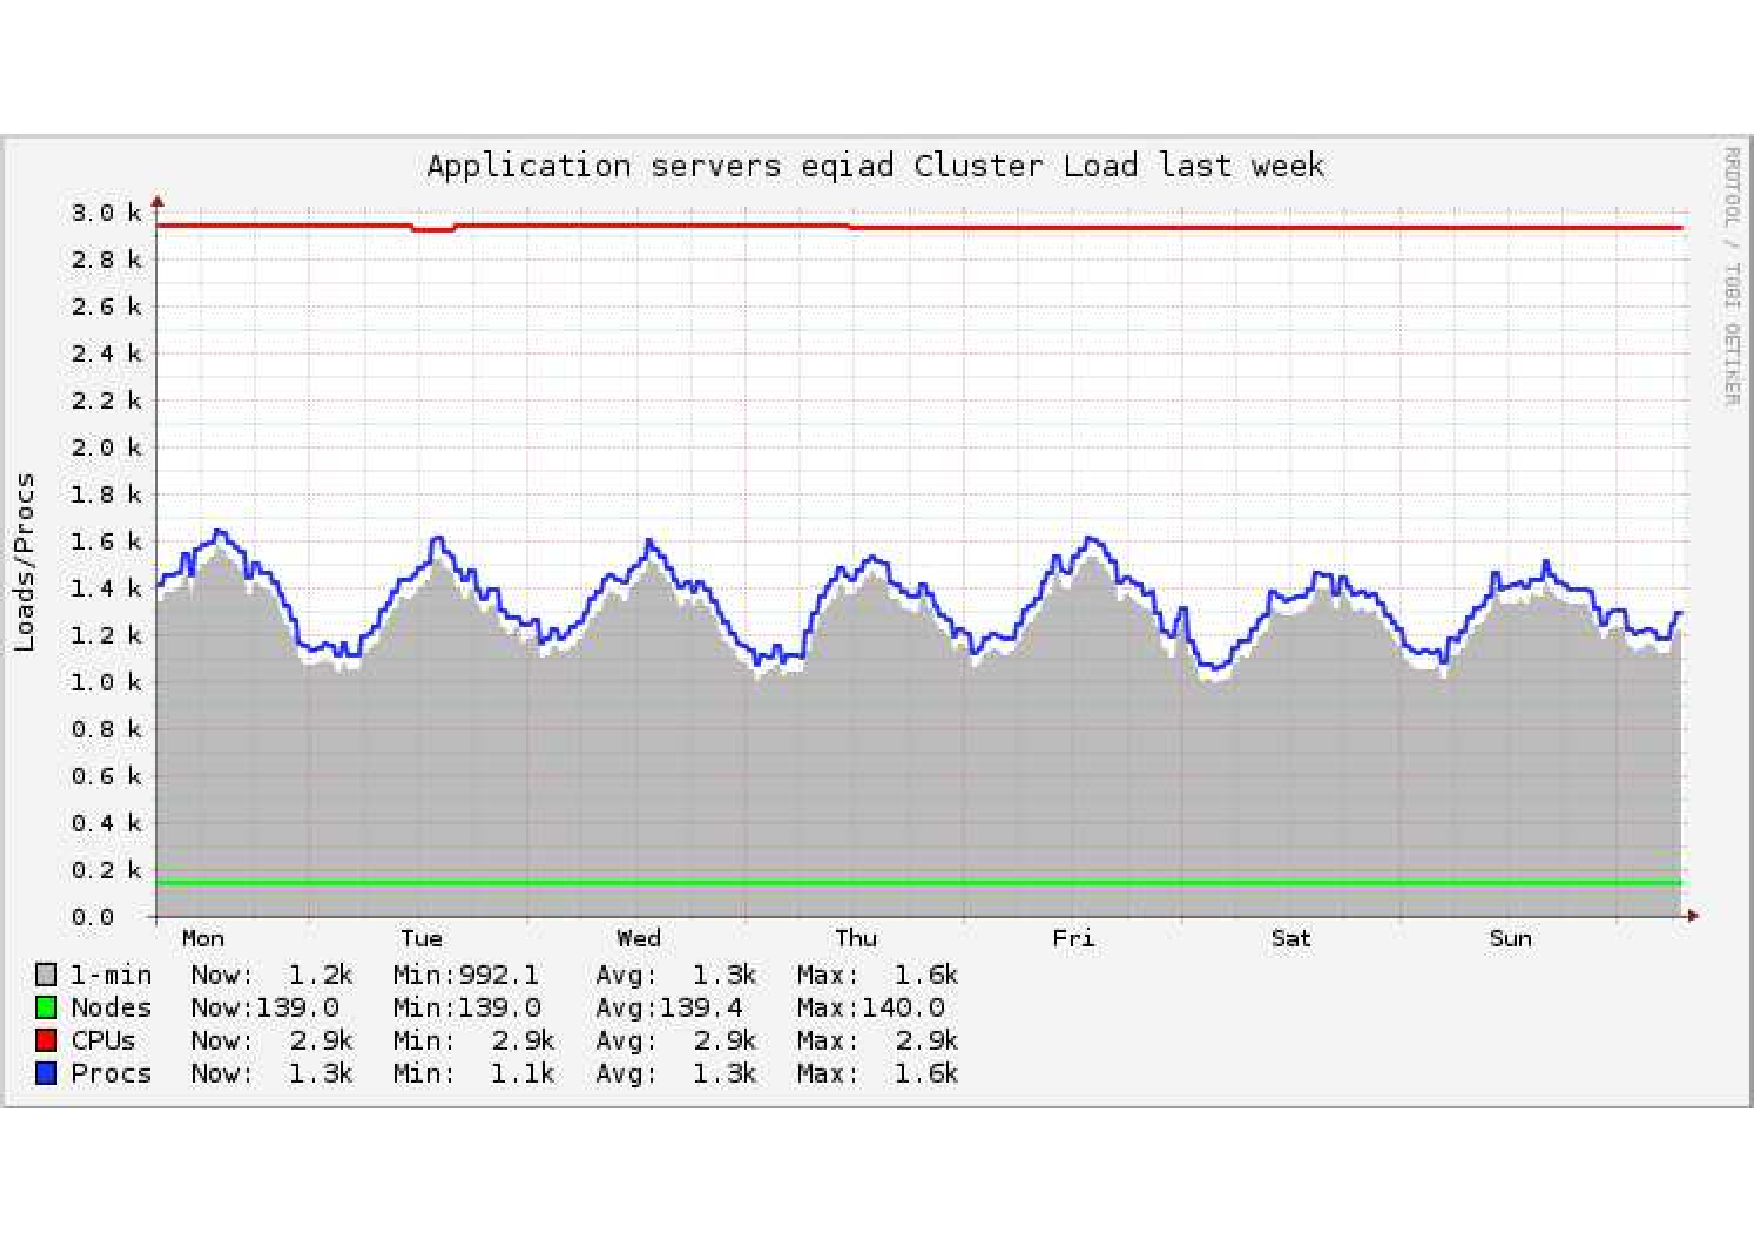
\includegraphics[width=\textwidth,keepaspectratio]{Figures/QueueingTheory/ganglia_app_server_18to24_Aug_2014.pdf}
\caption{Number of requests received by application servers during a week. 18-24 August 2014, Wikimedia Grid \cite{Ganglia_Wikimedia_Grid_Report} .}
\label{fig:ganglia_app_server_18to24_Aug_2014}
\end{figure}

\begin{figure}[!htbp]
\centering
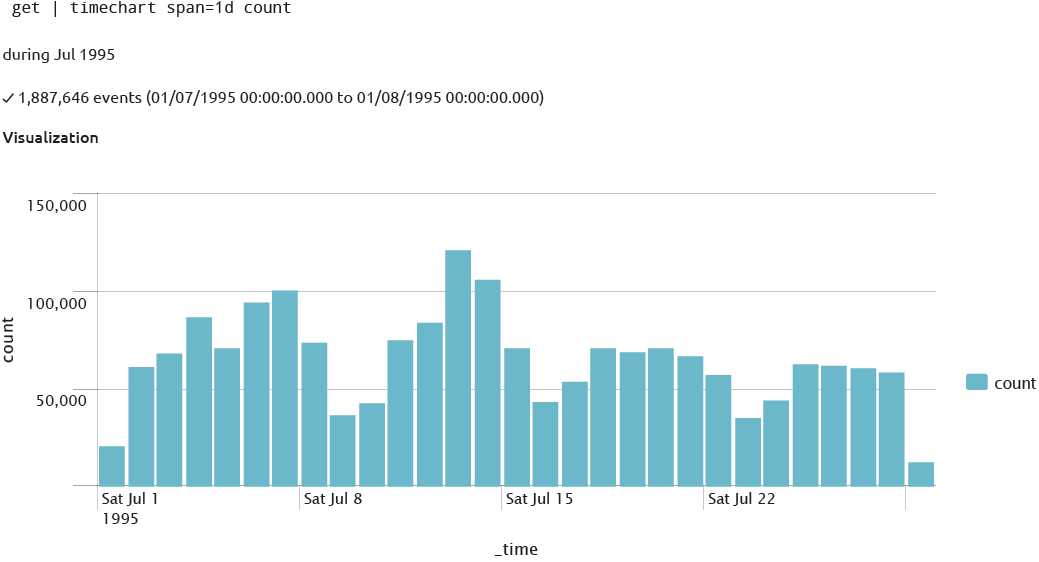
\includegraphics[width=\textwidth,keepaspectratio]{Figures/QueueingTheory/get.png}
\caption{Number of GET requests received by day \cite{plotly_ClarkNet-HTTP_get}, \cite{ClarkNet-HTTP}.}
\label{fig:_ClarkNet-HTTP_get}
\end{figure}

Incoming request rate in this workload varies depending on the day of the
week and the hour of the day. In our version of the
traces, there is a 12-hour difference between the peak (at noon)
and the trough (at midnight) in number of arriving requests, see Fig \ref{fig:ganglia_app_server_18to24_Aug_2014}.

In the simulation, random requests are generated according to:
\begin{equation}\label{eq:web_workload}
r = R_{min} + 0.5(R_{max} - R_{min}) + 0.5(R_{max} - R_{min}) sin(\frac{\pi t}{86400}) 
\end{equation}

Where 86400 is the number of seconds in a day (24 hours). $R_{max}$ is the maximum number of requests per second on that day, $R_{min}$ is the minimum number of requests of the day.

\subsubsection{Using the CloudHarmony API}

The CloudHarmony API provides an API for accessing different benchmark results for a
range of Cloud services [18]. The two relevant API endpoints are:
\begin{lstlisting}
https://www.cloudharmony.com/ws/getServicesWithBenchmark
benchmarkId
https://www.cloudharmony.com/ws/getServerBenchmarkResults
benchmarkId
serverId
lastBenchmarksOnly
\end{lstlisting}

The first endpoint lists the available Cloud services (and Cloud servers) that have been
benchmarked with the benchmarkId (mysql-bench:select and mysql-bench:insert), and the
second endpoint retrieves the benchmark results for all the Cloud servers that are passed as the
query parameters. Since we need the latest benchmark result, we also include the
‘lastBenchmarksOnly’ parameter in the query string. The API returns a JSON response that
can be parsed and utilised.

\subsection{Result}


\subsection{Database}

The mysql-bench benchmark suite is meant to tell any user what operations a given SQL implementation performs well or poorly. This benchmark is single-threaded, so it measures the minimum time for the operations performed. It measures the average time (in wallclock seconds) it takes for all of the mysql-bench benchmarks: alter-table, ATIS, big-tables, connect, create, insert, select, transactions and wisconsin. mysql-bench comprises of the following benchmarks:


\begin{enumerate}
  \item mysql-bench ATIS
  \item mysql-bench alter-table
  \item mysql-bench big-tables
  \item mysql-bench connect
  \item mysql-bench create
  \item mysql-bench insert
  \item mysql-bench select
  \item mysql-bench Wisconsin 
\end{enumerate}


In order to use these benchmark results to make useful decisions, we focus on the 2 most important query types – SELECT (READ) and INSERT (WRITE).The mysql-insert benchmark, at it’s core, issues 300,000 INSERT queries (if configured to run under default conditions) and calculates the total wall clock seconds to execute all queries. Thus if the wallclock seconds is, say t, on a particular system, we can deduce that the service rate of that server to process insert queries is $ \mu_w = \frac{300000}{t_w} $ queries/second. Similarly we can deduce the service rate for SELECT queries as $ \mu_r = \frac{1,194,631}{t_r} $ where the SELECT queries include the WHERE clause and thus SELECT queries with range parameters have been taken into account. This implies that if the fraction of READ/WRITE requests are given as $wr$ and $ww$, we can determine the average service rate as:

\begin{equation}\label{eq:db_workload}
\mu = wr \mu_r + ww \mu_w
\end{equation}

Thus using benchmark results and the READ/WRITE ratio, the service rate of different servers for performing MySQL queries can be computed.






